% 2013 重庆卷理科第 19 题：四棱锥 P-ABCD。
% PA⊥底面 ABCD；BC=CD=2，AC=4，∠ACB=∠ACD=60°，F 为 PC 中点。
% 底面按斜二测示意绘制：A 在左，B 在下，C 在右，D 在右上；AD、AC、BD 为不可见棱。
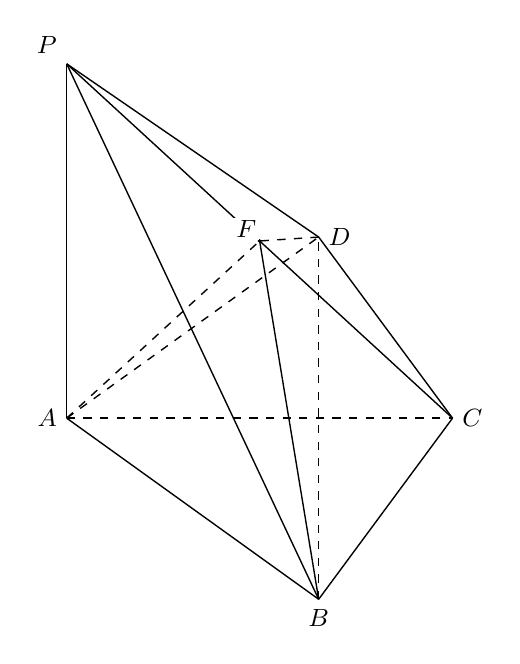
\begin{tikzpicture}[font=\small, line width=0.5pt, scale=1]
  \coordinate (A) at (0,0);
  \coordinate (P) at (0,4.5);
  \coordinate (B) at (3.2,-2.3);
  \coordinate (C) at (4.9,0);
  \coordinate (D) at (3.2,2.3);
  \coordinate (F) at (2.45,2.25);

  % 不可见棱
  \draw[dashed] (A) -- (D);
  \draw[dashed] (A) -- (C);
  \draw[dashed] (B) -- (D);
  % 可见棱
  \draw (P) -- (A);
  \draw (P) -- (B);
  \draw (P) -- (C);
  \draw (P) -- (D);
  \draw (A) -- (B);
  \draw (B) -- (C);
  \draw (C) -- (D);
  % F 在 PC 上；原页 AF、DF 为虚线，BF 为实线
  \draw[dashed] (A) -- (F);
  \draw (B) -- (F);
  \draw[dashed] (D) -- (F);
  \fill (F) circle (0.7pt);

  \node[above left] at (P) {$P$};
  \node[left] at (A) {$A$};
  \node[below] at (B) {$B$};
  \node[right] at (C) {$C$};
  \node[right] at (D) {$D$};
  \node[above left, fill=white, inner sep=1pt] at (F) {$F$};
\end{tikzpicture}
